\documentclass[10pt, conference, letterpaper]{IEEEtran}

\usepackage{algorithm}
\usepackage{algorithmicx}
\usepackage{algpseudocode}
\usepackage{amsfonts}
\usepackage{amsmath}
\usepackage{amssymb}
\usepackage[utf8]{inputenc} 
\usepackage{xcolor}
\usepackage{mathtools}
\usepackage{graphicx}
\usepackage{caption}
\usepackage{subcaption}
\usepackage{import}
\usepackage{multirow}
\usepackage{cite}
\usepackage[colorlinks=true, citecolor=blue, linkcolor=blue, urlcolor=blue]{hyperref}
\usepackage[export]{adjustbox}
\usepackage{breqn}
\usepackage{mathrsfs}
\usepackage{acronym}
%\usepackage[keeplastbox]{flushend}
\usepackage{setspace}
\usepackage{bm}
\usepackage{stackengine}
\usepackage{booktabs}
\usepackage{float}

\usepackage{listings}

\lstset{%
 backgroundcolor=\color[gray]{.85},
 basicstyle=\small\ttfamily,
 breaklines = true,
 keywordstyle=\color{red!75},
 columns=fullflexible,
}%

\lstdefinelanguage{BibTeX}
  {keywords={%
      @article,@book,@collectedbook,@conference,@electronic,@ieeetranbstctl,%
      @inbook,@incollectedbook,@incollection,@injournal,@inproceedings,%
      @manual,@mastersthesis,@misc,@patent,@periodical,@phdthesis,@preamble,%
      @proceedings,@standard,@string,@techreport,@unpublished%
      },
   comment=[l][\itshape]{@comment},
   sensitive=false,
  }

\usepackage{listings}

% listings settings from classicthesis package by
% Andr\'{e} Miede
\lstset{language=[LaTeX]Tex,%C++,
    keywordstyle=\color{RoyalBlue},%\bfseries,
    basicstyle=\small\ttfamily,
    %identifierstyle=\color{NavyBlue},
    commentstyle=\color{Green}\ttfamily,
    stringstyle=\rmfamily,
    numbers=none,%left,%
    numberstyle=\scriptsize,%\tiny
    stepnumber=5,
    numbersep=8pt,
    showstringspaces=false,
    breaklines=true,
    frameround=ftff,
    frame=single
    %frame=L
}

\renewcommand{\thetable}{\arabic{table}}
\renewcommand{\thesubtable}{\alph{subtable}}

\DeclareMathOperator*{\argmin}{arg\,min}
\DeclareMathOperator*{\argmax}{arg\,max}

\def\delequal{\mathrel{\ensurestackMath{\stackon[1pt]{=}{\scriptscriptstyle\Delta}}}}

\graphicspath{{./figures/}}
\setlength{\belowcaptionskip}{0mm}
\setlength{\textfloatsep}{8pt}

\newcommand{\eq}[1]{Eq.~\eqref{#1}}
\newcommand{\fig}[1]{Fig.~\ref{#1}}
\newcommand{\tab}[1]{Tab.~\ref{#1}}
\newcommand{\secref}[1]{Section~\ref{#1}}

\newcommand{\rev}[1]{{\color{blue}#1}}
\newcommand{\red}[1]{{\color{red}#1}}
\newcommand{\green}[1]{{\color[rgb]{0,0.6,0}#1}}
\newcommand{\mytexttilde}{{\raise.17ex\hbox{$\scriptstyle\mathtt{\sim}$}}}
\newcommand{\nasmarker}{^{\textcolor{blue}{\star}}}

%\renewcommand{\baselinestretch}{0.98}
% \renewcommand{\bottomfraction}{0.8}
% \setlength{\abovecaptionskip}{0pt}
\setlength{\columnsep}{0.2in}

% \IEEEoverridecommandlockouts\IEEEpubid{\makebox[\columnwidth]{PUT COPYRIGHT NOTICE HERE \hfill} \hspace{\columnsep}\makebox[\columnwidth]{ }} 

\title{Attention-Based PINN Solvers for Volterra Integro-Differential Equations}

\IEEEoverridecommandlockouts
\author{Federico Rossi$^\dag$
\thanks{$^\dag$Department of Physics, University of Padova}
\thanks{Source code repository available at: \url{https://github.com/Red-ux316/CrossPINN}}
}
\IEEEoverridecommandlockouts

\newcounter{remark}[section]
\newenvironment{remark}[1][]{\refstepcounter{remark}\par\medskip
   \textbf{Remark~\thesection.\theremark. #1} \rmfamily}{\medskip}

\begin{document}

\maketitle

\begin{abstract}

In the recent literature, standard Multi-Layer Perceptrons (MLPs) implementations of Physics-Informed Neural Networks (PINNs) have been used to solve complex Volterra Integro-Differential Equations (VIDEs). The intrinsic memory-dependent nature of such problems, however, suggests that transformer-like architectures could represent an inherently better-suited approach to this task. 
Starting from this idea, in this work we introduce CrossPINN (C-PINN), a query-based cross-attention architecture tailored for memory-dependent physical systems. By replacing heavy self-attention encoders with a learnable latent basis interrogated by spatial queries, C-PINN efficiently captures global Volterra integration kernels without quadratic computational overhead. 
Furthermore, integrating cross-attention as a global residual correction to a baseline MLP ($\hat{u} = \text{MLP} + \Delta u_{\text{Attn}}$) we where able to further improve the performance of the baseline model. In particular, evaluation on a benchmark set of Volterra problems—spanning 1D linear and non-linear VIDEs, coupled systems, and 2D viscoelastic PDE-IDEs—showed that C-PINN consistently outperforms pointwise MLP and RISN baselines, achieving up to an order of magnitude improvement in Mean Absolute Error (MAE).
\end{abstract}

\IEEEkeywords
PINN, Volterra equations, attention 
\endIEEEkeywords


% !TEX root = main.tex

\section{Introduction}
\label{sec:introduction}

Over the last decade, Deep Learning has been successfully employed to tackle complex physical systems traditionally governed by non-linear differential equations. Central to this paradigm are Physics-Informed Neural Networks (PINNs)~\cite{raissi2019physics}, which directly embed the governing physical laws into the training loss via differential reconstruction residuals. By penalizing non-physical predictions, PINNs enable the discovery of continuous, mesh-free solutions even when observational data is sparse.

While standard PINNs have proven to be highly effective for purely differential problems, significant progress can be made extending these frameworks to systems with non-local memory. In this work, we focus on Volterra Integro-Differential Equations (VIDEs), a complex class of physical problems where the unknown state is governed not only by its immediate derivatives but also by its entire historical trajectory through an integral operator. This non-local memory dependence is a fundamental property governing critical real-world phenomena, such as epidemiology models, population dynamics, and the behavior of viscoelastic materials.

Existing deep learning solvers for VIDEs, such as the Residual Integration Solver Network (RISN)~\cite{moghaddam2025risn}, rely on Multi-Layer Perceptron (MLP) variants. However, standard MLPs operate under a strict \textit{pointwise} paradigm, processing spatial coordinates independently. Because Volterra operators are dominated by causal memory, these pointwise architectures are structurally ill-suited to capture non-local dependencies. Lacking internal relational mechanisms, they are forced to delegate the entire memory correlation to the external loss formulation.

Motivated by recent advances in incorporating attention mechanisms into PINNs and operator learning (e.g., Physics-Guided Transformers~\cite{zeraatkar2026pgt}, PINNsFormer~\cite{zhao2023pinnsformer}, AttnPINNs~\cite{song2026attnpinns}, and operator-level attention frameworks~\cite{kissas2022learning}), we investigate whether attention-based models can better address VID equations. Nevertheless, standard Transformer architectures rely on full Self-Attention encoders,
which suffer from severe computational complexity that dramatically restricts their applicability in continuous physical problems. To overcome this computational bottleneck, we propose \textbf{CrossPINN (C-PINN)}~\cite{rossi2026crosspinn}, an efficient architecture that bypasses dynamic sequence encoding in favor of a direct, learnable global latent basis interlinked via Sequential Cross-Attention.
While established complementary techniques—such as ReLoBRaLo loss balancing, Gauss-Legendre quadrature, and positional encodings—are directly adopted from the literature, our primary focus remains on isolating and evaluating the cross-attention mechanism itself as a solver for VIDEs.
The primary contributions of our implementation are the following:
\begin{itemize}
    \item We designed and implemented \textbf{CrossPINN (C-PINN)}, a domain-wise Cross-Attention architecture tailored to model non-local memory in Volterra operators via a direct learnable global latent basis.
    \item We documented the architectural evolution of the framework, detailing the iterative design choices required to adapt standard attention mechanisms to the strict constraints of physics-informed solvers.
    \item We performed a systematic benchmark evaluation comparing C-PINN variants against baseline MLP architectures across representative Volterra problems.
\end{itemize}

This report is structured as follows. Section~\ref{sec:background} reviews the VIDE mathematical formulation and related work. Section~\ref{sec:processing_pipeline} details the query-based processing pipeline and spatial coordinate streams. Section~\ref{sec:learning_framework} presents the C-PINN architecture and optimization strategies. Finally, Section~\ref{sec:results} discusses the benchmark results, followed by concluding remarks in Section~\ref{sec:conclusions}.

% !TEX root = main.tex

\section{Background and Related Work}
\label{sec:background}

\subsection{Problem Formulation and Physics-Informed Loss}
A general non-linear Volterra Integro-Differential Equation (VIDE) defined on the standard bounded domain $\Omega = [a, b]$ is formulated as:
\begin{equation}
    \begin{aligned}
        \mathcal{D}(u)(x) + \mathcal{F}(u)(x) 
        = \mathcal{S}(x) + \int_{a}^{x} K(x, y) \, \zeta\big(u(y)\big) \, dy,
    \end{aligned}
    \label{eq:general_vide}
\end{equation}
where $\mathcal{D}(u)(x)$ represents a linear differential operator, $\mathcal{F}(u)(x)$ denotes local algebraic state interactions, $K(x, y)$ is a continuous memory kernel, $\zeta(\cdot)$ is a non-linear mapping, and $\mathcal{S}(x)$ is a known driving source. 

To train a neural approximator $\hat{u}_\theta(x)$, we minimize the Integro-Differential Equation (IDE) residual $ \mathcal{R}(x)$ of Eq.~\eqref{eq:general_vide}. Evaluating this residual requires computing the Volterra integral, which we discretize via an $N_q$-point Gauss-Legendre quadrature scheme~\cite{moghaddam2025risn,aghaei2024pinnies}, yielding the computable residual $\mathcal{R}(x)$:
\begin{equation}
    \begin{aligned}
        \mathcal{R}(x) = \;&\mathcal{D}(\hat{u}_\theta)(x) + \mathcal{F}(\hat{u}_\theta)(x) \\
        &- \sum_{j=1}^{N_q} w_j(x) K(x, y_j) \, \zeta\big(\hat{u}_\theta(y_j)\big) - \mathcal{S}(x),
    \end{aligned}
    \label{eq:coupled_residual}
\end{equation}
where $y_j$ and $w_j(x)$ represent the quadrature nodes and integration weights. The network parameters $\theta$ are optimized by minimizing the Mean Squared Residual $\mathcal{L}_{\text{IDE}} = \frac{1}{N_r} \sum_{i=1}^{N_r} | \mathcal{R}(x_i) |^2$ over a batch of $N_r$ collocation points.

\subsection{Volterra Solvers and Manufactured Solutions}

In recent years, several specialized deep learning architectures have been introduced to solve integral and integro-differential equations, including Auxiliary PINNs (A-PINN)~\cite{yuan2022apinn}, and internal variable reformulations for exponential kernels~\cite{Jang_2026}. Notably, Moghaddam et al.~\cite{moghaddam2025risn} proposed the Residual Integration Solver Network (RISN) to mitigate gradient degradation in integral operators.

Unlike standard machine learning tasks, forward operator learning often lacks experimental observational datasets. To rigorously validate architectures without real-world data, we employ the Method of Manufactured Solutions (MMS)~\cite{moghaddam2025risn}. In MMS, a smooth analytical target solution $u_{\text{exact}}(x)$ is selected \textit{a priori} and substituted into the integro-differential operator to analytically synthesize the corresponding source term $\mathcal{S}(x)$. 
This guarantees to have an exact objective to use for precise and reliable error quantification against baseline architectures.

While RISN and related variants provide structural improvements over standard baseline Multi-Layer Perceptrons, applying an MLP-based architecture to solve Eq.~\eqref{eq:coupled_residual} introduces a structural mismatch, which we refer to as the \textit{pointwise paradox}. Volterra equations are intrinsically non-local, yet MLPs evaluate each coordinate in strict isolation, delegating the entire sequence-awareness to the external loss function.

We hypothesize that this structural mismatch gives rise to an important optimization pathology, which we call the \textit{gradient conflict}. As shown in Eq.~\eqref{eq:coupled_residual}, computing the numerical residual $\mathcal{R}(x)$ mathematically couples the network's prediction at the present coordinate, $\hat{u}_\theta(x)$, with its predictions at historical quadrature nodes, $\hat{u}_\theta(y_j)$. During backpropagation, the optimizer must update the shared global weights $\theta$ based on these coupled outputs. Consequently, the gradients computed for the local state $\hat{u}_\theta(x)$ can directly conflict with those required to minimize approximation errors across past states $\hat{u}_\theta(y_j)$, trapping the optimizer in suboptimal local minima.

\subsection{Resolving the Paradox via Attention}
Tom mitigate this potential gradient conflict, we propose embedding a Cross-Attention mechanism into the physics-informed architecture. Because cross-attention is intrinsically set-aware, it allows the model to correlate a specific query coordinate (the present state) with a structured latent basis (the historical memory) during the forward pass, embedding memory integration directly into the network architecture.

% !TEX root = main.tex

\section{Query-Based Processing Pipeline and Data Streams}
\label{sec:processing_pipeline}

To model non-local Volterra operators while preserving computational efficiency, C-PINN processes spatial coordinates through a query-based processing pipeline, as illustrated in Fig.~\ref{fig:c_pinn_macro_arch}. Rather than treating input coordinates as isolated point samples, physical coordinates act as functional sets of queries that interrogate a globally structured latent basis (see Section~\ref{sec:learning_framework} for detailed micro-architectural specifications of the decoder stack).

\subsection{Functional Coordinate Streams and Discretization}
Under the Method of Manufactured Solutions (MMS)~\cite{moghaddam2025risn}, spatial coordinates are sampled directly from the physical domain and formatted into four distinct functional sets:
\begin{enumerate}
    \item \textbf{Support Anchors ($X_{sup}$):} A grid of $N_{sup}$ equidistant coordinates spanning $[a, b]$, serving as static spatial anchors for the global latent basis.
    \item \textbf{Collocation Queries ($X_r$):} A batch of $N_r$ domain points sampled at random at each iteration to compute differential operator residuals $\mathcal{R}(x)$.
    \item \textbf{Quadrature Queries ($X_q$):} For each collocation point $x_i \in X_r$, $N_q$ historical coordinates $\{y_j(x_i)\} \subset [a, x_i]$ are generated as mapped Gauss-Legendre quadrature roots to evaluate Volterra integrals. 
    \item \textbf{Boundary Queries ($X_{bc}$):} A set of $N_{bc}$ boundary/initial coordinates enforcing Dirichlet or initial condition constraints.
\end{enumerate}
While domain-adapted sampling distributions (e.g., Beta distributions) could be used to concentrate collocation points near boundaries or stiff regions, for simplicity we adopt uniform grid sampling across all experimental evaluations.

\subsection{Encoder Omission and Non-Local Projection}
Standard Transformer architectures rely on encoder stacks with $\mathcal{O}(N^2)$ Self-Attention complexity to build contextual sequence representations. Inspired by Perceiver IO~\cite{jaegle2021perceiverio}, C-PINN explicitly omits the Self-Attention encoder, since introduces heavy computational overhead without proportional gains in physical expressivity. Instead, the spatial domain is anchored to the static Support Anchors ($X_{sup}$), forming a \emph{Global Latent Basis}. Target query coordinates $X_Q \in \{X_r, X_q, X_{bc}\}$ evaluate solution values via targeted Cross-Attention layers. This operation acts as a \emph{Learnable Non-Local Projection}: query coordinates compute similarity scores across the latent basis, retrieving integrated historical context in a single forward pass while bypassing the gradient conflict inherent to pointwise MLPs.

\subsection{Metric Integrity via Shared Positional Encoding}
Maintaining physical metric integrity across the attention mechanism is essential for accurate spatial regression. In C-PINN, both the physical queries $X_Q$ and the static support anchors $X_{sup}$ are embedded using the exact same Positional Encoder $E_{pos}(\cdot)$. Sharing these weights guarantees that dot-product similarity metrics in the latent space ($Q \cdot K^T$) directly reflect physical geometric distances in the original domain, preventing spatial distortions during attention weighting.

%\input{data_rep}

% !TEX root = main.tex

\section{Learning Framework}
\label{sec:learning_framework}

Designing a physics-informed attention mechanism requires balancing expressive non-local capacity with optimization stability. The C-PINN learning framework builds upon a custom un-normalized Cross-Attention module connected to a symmetric global latent basis. Architectural and training hyperparameters were systematically selected via hyperparameter tuning using Optuna's Tree-structured Parzen Estimator (TPE) paired with Median Pruning. Key Optuna-tuned components are indicated by a blue star marker ($\nasmarker$).

\begin{figure*}[t]
    \centering
    \begin{subfigure}{\textwidth}
        \centering
        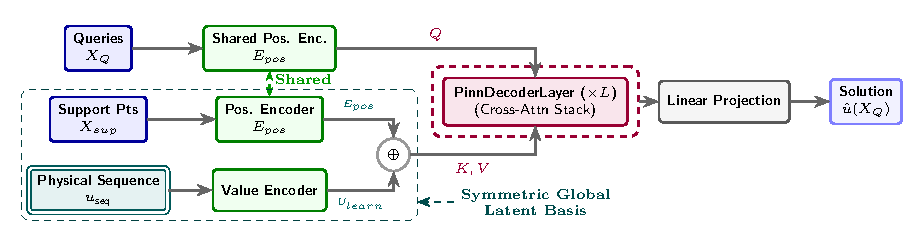
\includegraphics[width=0.92\textwidth]{figures/tlp_architecture.pdf}
        \caption{Overall macro-architecture of CrossPINN (C-PINN), depicting the baseline MLP stream interlinked with the Cross-Attention memory corrector.}
        \label{fig:c_pinn_macro_arch}
    \end{subfigure}
    \vspace{0.3cm}
    \begin{subfigure}{\textwidth}
        \centering
        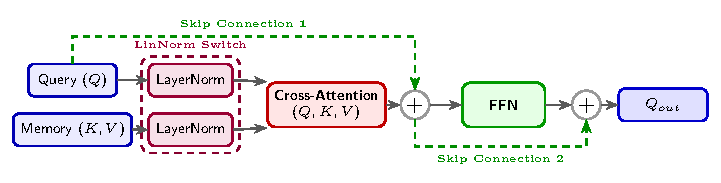
\includegraphics[width=0.92\textwidth]{figures/modules_architecture.pdf}
        \caption{Detailed micro-architecture of the custom \texttt{PinnDecoderLayer}, highlighting the optional LinNorm query/key normalization switch and un-normalized residual skip connections.}
        \label{fig:pinn_decoder_layer_micro}
    \end{subfigure}
    \caption{Complete schematic representation of the C-PINN framework: (a) Macro-scale hybrid architecture; (b) Micro-scale \texttt{PinnDecoderLayer} building block.}
    \label{fig:c_pinn_full_architecture}
\end{figure*}

\subsection{Symmetric Global Latent Basis}
To model historical memory in Volterra operators, spatial queries attend to a globally accessible latent memory matrix. Rather than decoupling spatial coordinates from latent states, C-PINN constructs a symmetric joint spatial-latent basis~\cite{jaegle2021perceiverio}:
\begin{equation}
    \text{Memory} = E_{pos}(X_{sup})\nasmarker + U_{learn} \in \mathbb{R}^{N_{sup} \times H},
    \label{eq:latent_basis}
\end{equation}
where $E_{pos}(X_{sup})$ provides deterministic positional embeddings for spatial support anchors $X_{sup}$, and $U_{learn} \in \mathbb{R}^{N_{sup} \times H}$ is a latent value matrix representing the solution basis over the support anchors. Summing spatial and value representations ensures content-aware attention: queries $X_Q$ attend to historical states based on both physical proximity and latent solution characteristics.

\subsection{Latent Solution Parameterization and Dynamic Warm-Start}
To force a physical interpretation of $U_{learn} \in \mathbb{R}^{N_{sup} \times H}$ as a latent solution basis over the domain, we structure the matrix using a spatial solution sequence $u_{\text{seq}}(X_{sup}) = \text{MLP}(X_{sup}) \in \mathbb{R}^{N_{sup} \times 1}$ evaluated by a pre-trained baseline MLP at the support anchors, projected via a linear value encoder $\text{ValEnc}(\cdot)$:
\begin{equation}
    U_{learn} = \text{ValEnc}(u_{\text{seq}}) = u_{\text{seq}} W_{val} + b_{val}.
\end{equation}

During the initial phase of training, the solution sequence $u_{\text{seq}}$ is kept frozen to the baseline MLP values for a set number of epochs ($E_{\text{unfreeze}}\nasmarker$). This allows the network to first optimize the attention mechanism and positional encodings around the baseline physical field before fine-tuning the solution representation itself.

Since we could not determine \textit{a priori} whether optimizing the 1D physical sequence or the full 2D latent matrix was superior, we let Optuna select between two unfreezing parameterization modes$\nasmarker$:
\begin{enumerate}
    \item \textbf{Sequence Parameterization:} Unfreezes the 1D physical sequence $u_{\text{seq}} \in \mathbb{R}^{N_{sup} \times 1}$, which is projected through the learnable $\text{ValEnc}(\cdot)$ layer.
    \item \textbf{Direct Latent Matrix Parameterization:} Unfreezes the full $N_{sup} \times H$ matrix $U_{learn}$ directly, granting the optimizer maximum feature capacity for high-dimensional residual refinement.
\end{enumerate}

Furthermore, because initializing $U_{learn}$ with MLP ``hints'' introduces a strong physical inductive bias that might either accelerate convergence or excessively restrict representation capacity, we left the activation of Warm-Start as an explicit Neural Architecture Search (NAS) dimension$\nasmarker$. If Warm-Start is disabled, $U_{learn}$ is initialized randomly and trained end-to-end from epoch 1.

\subsection{Positional Encoding Variants}
To map continuous spatial coordinates into high-dimensional latent space without spectral bias, C-PINN leverages a positional encoder $E_{pos}(\cdot)\nasmarker$. Rather than hardcoding a single structure, the NAS space includes five standard encoding mechanisms adopted directly from literature:
\begin{itemize}
    \item \textbf{Random Fourier Features (RFF):} Projects coordinates using a static Gaussian frequency matrix to enforce isotropic spatial distance metrics.
    \item \textbf{Learnable Fourier Features (LFF):} Dynamically optimizes spatial frequency bands via backpropagation.
    \item \textbf{MLP Encoder:} A standard two-layer feedforward network with GELU activations for generic non-linear spatial mapping.
    \item \textbf{Sinusoidal MLP (SIREN):} Employs periodic activations with a tunable scale hyperparameter $\omega_0\nasmarker$ to capture high-frequency physical gradients.
    \item \textbf{Radial Basis Functions (RBF):} Maps coordinates relative to learnable Gaussian centers and scale factors for localized spatial activations.
\end{itemize}

\subsection{Custom Cross-Attention and Decoder Stack}
Standard PyTorch Transformer layers (\texttt{nn.TransformerDecoderLayer}) enforce external LayerNormalization on hidden features and residual skip connections, while \texttt{nn.MultiheadAttention} lacks mechanisms to selectively normalize Query and Key projections. In physics-informed regression, applying LayerNorm across spatial feature dimensions forces activations to zero mean and unit variance, destroying absolute spatial scales and dampening higher-order Autograd derivatives.

To resolve these limitations, we designed a custom decoder architecture featuring two normalization controls:
\begin{enumerate}
    \item \textbf{Residual LayerNorm Removal:} External LayerNorm operations on decoder inputs and skip connections are replaced with identity mappings, preserving uncorrupted physical solution magnitudes and derivative scales.
    \item \textbf{Query/Key Normalization Switch:} To evaluate whether normalizing Query ($Q = Q W_Q$) and Key ($K = K W_K$) projections stabilizes logit dynamics, we introduced an internal query/key normalization switch as a NAS dimension$\nasmarker$.
\end{enumerate}

When query and key normalization is disabled, raw geometric inner products drive attention scoring:
\begin{equation}
    \text{Attn}(Q, K, V) = \text{Softmax}\left(\frac{(Q W_Q) (K W_K)^T}{\sqrt{d_k}}\right) V W_V.
    \label{eq:linnorm_attn}
\end{equation}
While the codebase supports lower-triangular causal attention masking ($y_j \le x$), causal masking was left unconstrained in our primary benchmark evaluations.

The complete Cross-Attention decoder comprises a stack of $L\nasmarker$ identical decoder layers ($L \in [1, 4]$ tuned via Optuna). Within each layer, intermediate feature representations pass through the Cross-Attention block followed by a Feed-Forward Network (FFN), with internal residual skip connections bypassing both blocks to guarantee stable gradient propagation through deep decoder stacks (Fig.~\ref{fig:c_pinn_full_architecture}b). Finally, the refined latent features $Q_{\text{lat}} \in \mathbb{R}^{M \times H}$ exiting the decoder stack are projected back to the physical solution space via a simple linear projection layer ($\text{Linear}: \mathbb{R}^H \to \mathbb{R}^1$).

\subsection{MLP-Residual Correction Framework}
To combine the strong inductive bias of MLPs for local differential dynamics with the non-local integration capacity of attention, C-PINN formulates the hybrid residual architecture$\nasmarker$:
\begin{equation}
    \hat{u}_\theta(x) = \text{MLP}(x) + \Delta u_{\text{Attn}}(x),
\end{equation}
where $\text{MLP}(x)$ models the macroscopic physical field and $\Delta u_{\text{Attn}}(x)$ predicts fine-grained Volterra memory corrections (Fig.~\ref{fig:c_pinn_full_architecture}a).

\subsection{Optimization Strategy and Hyperparameter Search Space}
Training is performed by minimizing a composite loss function balancing differential/integral residuals and boundary constraints:
\begin{equation}
    \mathcal{L}_{\text{total}} = \mathcal{L}_{\text{IDE}} + \lambda_{\text{BC}} \mathcal{L}_{\text{BC/IC}}.
\end{equation}
To prevent gradient dominance between loss components, constraint weight $\lambda_{\text{BC}}$ is dynamically updated using Relative Loss Balancing with Random Lookback (ReLoBRaLo)~\cite{relobralo2021}. Smooth $C^\infty$ activation functions$\nasmarker$ ($\text{activation} \in \{\text{GELU}, \text{Tanh}, \text{SiLU}\}$) are employed across all layers to ensure continuous Autograd derivatives without non-physical singularities.

Optimization is performed using the AdamW optimizer. Optimization is bounded by a maximum of $10,000$ epochs paired with an Early Stopping mechanism (patience of $500$ epochs, minimum delta threshold of $10^{-5}$).

Architectural hyperparameter optimization is conducted systematically using Optuna TPE across the search space:
\begin{itemize}
    \item \textbf{Latent Dimensions ($H$):} $H \in \{32, 64, 128\}$.
    \item \textbf{Attention Heads ($h$):} $h \in \{2, 4, 8\}$ (constrained such that $H \bmod h = 0$).
    \item \textbf{Decoder Layers ($L$):} $L \in \{1, 2, 3, 4\}$.
    \item \textbf{Support Anchors ($N_{\text{sup}}$):} $N_{\text{sup}} \in \{32, 64, 128\}$.
    \item \textbf{Learning Rate ($\text{lr}$):} Log-uniform float $\text{lr} \in [5 \times 10^{-4}, 5 \times 10^{-2}]$.
    \item \textbf{Weight Decay ($\text{wd}$):} Log-uniform float $\text{wd} \in [10^{-6}, 10^{-4}]$.
    \item \textbf{Warm-Start Unfreeze Epoch ($E_{\text{unfreeze}}$):} $E_{\text{unfreeze}} \in \{2, 1000, 2000, 3000\}$.
\end{itemize}

% !TEX root = main.tex

\section{Experimental Results and Analysis}
\label{sec:results}

\begin{table*}[t]
\centering
\resizebox{\textwidth}{!}{
\begin{tabular}{@{}lllc@{}}
\toprule
\textbf{ID} & \textbf{Category} & \textbf{Operator Formulation} & \textbf{Exact Solution $u(x)$} \\ 
\midrule
\textbf{Prob A} & 1D Linear (2nd Kind) & $u(x) = S(x) + \int_0^x (t-x) u(t) dt$ & $x + e^x$ \\
\textbf{Prob B} & 1D IDE (1st Order) & $u'(x) = S(x) + \int_0^x u(t) dt$ & $\sin(x)$ \\
\textbf{Prob C} & 1D Non-Linear IDE & $u'(x) = S(x) + \int_0^x u^2(t) dt$ & $x$ \\
\textbf{Prob D} & 1D IDE (2nd Order) & $u''(x) = S(x) + \int_0^x (x-t) u(t) dt$ & $\sin(x)$ \\
\textbf{Prob E} & 2D Viscoelastic PDE & $\partial_t u = \alpha \partial_{xx} u + S(x,t) - \gamma \int_0^t e^{-\beta(t-s)} u(x,s) ds$ & $\sin(\pi x)e^{-t}$ \\
\textbf{Prob F} & 1D Coupled IDE System & $\begin{cases} u_1'(x) = S_1(x) + \int_0^x [(x-t)u_1(t) + (x-t+1)u_2(t)] dt \\ u_2'(x) = S_2(x) + \int_0^x [(x-t+1)u_1(t) + (x-t)u_2(t)] dt \end{cases}$ & $\begin{cases} u_1(x) = 1+x+x^2 \\ u_2(x) = 1-x-x^2 \end{cases}$ \\
\bottomrule
\end{tabular}}
\caption{Benchmark Suite of Volterra Integro-Differential Equations (Note that all our problems are defined on $\Omega = [0,1]$).}
\label{tab:equations_suite}
\end{table*}

\subsection{Evaluation Protocol}
Inferential accuracy is evaluated on an independent, dense uniform test grid of $N_{\text{test}} = 1000$ coordinates spanning $[a, b]$, quantified via Mean Absolute Error (MAE) against the analytical ground truth solution $u_{\text{exact}}(x)$ synthesized via MMS. While both the total optimization loss ($\mathcal{L}_{\text{Total}}$) and the absolute physical error (MAE) were rigorously tracked, we report the MAE as the primary metric for comparative analysis, as it provides a standardized, unbiased measure of spatial generalization across equations with varying residual scales.

\subsection{Benchmark Suite and Physical Formulations}
To systematically validate the C-PINN architecture against baseline models, we selected a diverse suite of Volterra Integro-Differential Equations. The benchmark includes foundational 1D formulations (Prob A, B, C, D)~\cite{moghaddam2025risn}, a 2D spatio-temporal viscoelastic PDE (Prob E)~\cite{Jang_2026}, and a coupled system of integro-differential equations (Prob F)~\cite{moghaddam2025risn}. Due to space constraints, the governing operators, integration kernels, and analytical ground truths are summarized in Table~\ref{tab:equations_suite}.

\subsection{Ablation Study and Performance Analysis}
Table~\ref{tab:results_mae} summarizes the inferential accuracy (MAE) comparing the baseline models (MLP and RISN) against C-PINN with and without the global residual skip connection.

For scalar 1D benchmarks (Prob A, B, C, D), the full C-PINN architecture consistently outperforms both baselines and the no-skip variant, reducing MAE by up to an order of magnitude. We hypothesize that the global skip connection structurally decouples the learning objective: the baseline MLP captures the primary differential field, while the cross-attention mechanism strictly models non-local memory corrections.

Conversely, for the coupled IDE system (Prob F), C-PINN without the skip connection achieves the best overall performance ($7.35 \times 10^{-5}$). We conjecture that in multi-component coupled systems, constraining the architecture with an MLP residual base may introduce optimization stiffness, whereas unconstrained latent attention resolves the coupled field more effectively.

Finally, for the 2D spatio-temporal viscoelastic PDE (Prob E), C-PINN does not outperform the specialized RISN baseline ($5.37 \times 10^{-4}$ vs. $1.37 \times 10^{-4}$). While C-PINN demonstrates strong superiority on simpler 1D benchmarks, this outcome suggests that scaling latent cross-attention to complex, higher-dimensional spatio-temporal systems poses significant challenges, likely requiring further architectural modifications and deeper investigation.

Detailed training loss curves and solution fit profiles across all problems are omitted here as they offer limited additional insight beyond primary MAE metrics, but complete visualization reports and trained model weights are publicly available in the project repository~\cite{crosspinn_drive2026}.

\begin{table}[H]
\centering
\resizebox{\columnwidth}{!}{
\begin{tabular}{@{}lcccc@{}}
\toprule
 & \textbf{MLP} & \textbf{RISN} & \textbf{C-PINN} & \textbf{C-PINN} \\ 
\textbf{Problem} & Baseline & Baseline & (No Skip) & (Global Skip) \\ \midrule
\textbf{Prob A} & 2.23e-02 & 1.04e-03 & 4.21e-03 & \textbf{5.42e-04} \\
\textbf{Prob B} & 5.42e-04 & 1.48e-04 & 3.74e-05 & \textbf{8.86e-06} \\
\textbf{Prob C} & 5.10e-05 & 4.56e-05 & 2.81e-05 & \textbf{3.37e-06} \\
\textbf{Prob D} & 1.56e-05 & 7.05e-06 & 4.41e-05 & \textbf{1.31e-06} \\
\textbf{Prob E} & 6.76e-04 & \textbf{1.37e-04} & 3.32e-03 & 5.37e-04 \\
\textbf{Prob F} & 2.97e-04 & 2.31e-04 & \textbf{7.35e-05} & 2.65e-04 \\ \bottomrule
\end{tabular}}
\caption{Mean Absolute Error (MAE) Benchmark Comparison}
\label{tab:results_mae}
\end{table}

\subsection{Neural Architecture Search (NAS) Insights}
Neural Architecture Search reveals distinct optimization dynamics between the residual and non-residual framework variants. 

When the global residual skip connection is active, Optuna displays broad flexibility across structural choices without a single dominant configuration. Notably, base-model latent initialization shows no strict preference, indicating that the cross-attention mechanism can effectively learn the latent memory basis autonomously. This insensitivity highlights the robustness of the residual formulation: since the baseline MLP absorbs the primary spatio-temporal dynamics, the attention stream remains stable across hyperparameter choices, consistently favoring shallow decoder stacks ($1$--$2$ layers) paired with multi-head attention ($h = 4$ or $8$).

Conversely, when the skip connection is disabled, resolving both differential and integral dynamics end-to-end imposes tighter constraints. In this setting, Optuna consistently rejects layer normalization to preserve metric gradients and requires high-density memory support (128 support points), confirming that unconstrained attention dynamics demand strict metric preservation.


% !TEX root = main.tex

\section{Conclusions and Future Work}
\label{sec:conclusions}

In this work, we introduced CrossPINN (C-PINN), a query-based cross-attention architecture designed to tackle non-local memory dependencies in Volterra Integro-Differential Equations (VIDEs). By representing continuous physical coordinates as queries that interrogate a learnable latent memory basis, C-PINN overcomes the inherent pointwise limitations of standard MLPs while bypassing the quadratic computational burden of self-attention encoders.

Empirical evaluations across diverse Volterra benchmarks demonstrate the flexibility of the proposed framework. On scalar 1D problems, C-PINN with global residual skip connections delivers up to an order of magnitude error reduction over standard baselines. In coupled system settings, removing the skip connection effectively relieves optimization stiffness between interacting fields. Finally, performance on spatio-temporal formulations underscores both the potential and current boundaries of latent cross-attention, pointing toward promising directions for higher-dimensional operator modeling.

Furthermore, Neural Architecture Search (NAS) reveals no strict preference for any specific architectural choices, confirming the overall structural stability and robustness of the proposed framework.

Future research directions could explore extending the framework to more complex physical formulations, evaluating alternative data and domain management strategies such as time-marching, and investigating the operator learning capabilities of C-PINN to generalize across parametric memory kernels. The complete source code implementation, model architectures, and benchmark suite are made publicly available at \url{https://github.com/Red-ux316/CrossPINN}.




\bibliographystyle{IEEEtran}
\bibliography{references}

\end{document}


